\documentclass[letterpaper, 10pt]{article}
\usepackage[headings]{fullpage}
\usepackage{amsmath, amsthm, amssymb, fancyhdr, mathptmx, enumerate}
\usepackage[pdftex]{graphicx}
\include{mathmacros}

\pagestyle{fancy}
\headheight 23pt
\lhead{Daniel Sommermann, Michael Gummelt}
\chead{CS240H, Hindsight Debugging}

\title{Hindsight Debugging \\
CS 240H: Functional Systems in Haskell}
\date{16 December 2011}
\author{
  \begin{tabular}{c c}
    Michael Gummelt & Daniel Sommermann \\
    \texttt{mgummelt@cs.stanford.edu} &
    \texttt{dcsommer@cs.stanford.edu}
  \end{tabular}
}
\newcommand{\ttt}{\texttt}

\begin{document}

\maketitle

\section{Abstract}
For this project we decided to explore the feasibility of a ``hindsight
debugger.'' Consider the following scenario: a programmer wants to debug a
piece of code, but isn't certain exactly where it goes
wrong. Traditionally, the programmer would have to set a breakpoint at
some arbitrary point and step through the code until some computation is
made that the programmer recognizes as invalid. If the programmer realizes
at a later point that the error was earlier, the debugging process must be
started once again, re-running the code, to hopefully catch the bug the
next time around.

In our debugger, we simplify this process by allowing inspection of the
stack on any line of code. In particular, our debugger allows the
programmer to inspect all stacks that existed while executing a particular
line of code. This way, a programmer can jump around to quickly pinpoint
the source of the error without being constrained by the semantics of 
debugging a live, running program.

To make our proof of concept debugger, we defined a simple language (MGDS)
that has functions, assignment, and integer arithmetic. We parse source
files using Parsec into an AST. Then, a specialized interpreter is run
over the AST, mapping line numbers to stacks. Finally, a debug loop is
entered wherein the user can query for stack and variable information for
any line of code. 

\section{Previous Work}
Microsoft's Visual Studio is the only other product we are aware of that
has similar functionality at the time of this writing, however, this
feature, called by Microsoft ``IntelliTrace,'' is only available in the
most expensive version of Visual Studio, which retails for over twelve
thousand dollars per license.

IntelliTrace is of course more fully-featured compared to our
work. IntelliTrace is also mostly geared towards debugging other people's
crashes which are hard to reproduce. The client would enable IntelliTrace
and generate a more complete log file that would be sent to the
responsible party for debugging.

\section{Language Definition for MGDS}
The BNF of our language is given below
\begin{verbatim}
f = fn(x1, .., xn) { s; [s;] }

s = var = e
    return e
    returnif e, e

e = c1 | ... | cn (constants)
    (e)
    x
    e1 + e2
    e1 - e2
    e1 * e2
    e1 / e2
    e1 == e2
    !e1
    e1 && e2
    e1 || e2
    e1 == e2
    e1 < e2
    e1 > e2
    if e1 then e2 else e3
    f(e1, ..., en)
\end{verbatim}
MGDS is not a strictly pure language since it allows you to assign to the
same variable twice in one function. Arguments are passed by value during
function invocation, so the previous case is the only impure part of the
language. Also, there is no branching (besides early return via the
\ttt{returnif} operator) or looping in our language. The choice to omit
these constructs allowed us to quickly develop our debugger and
language. It also simplifies our model, since with loops, the same line of
code could be executed many, many times for a single function call. It is
a solvable problem (run the function body and the loop as many times as
the user specifies), but we leave this UI work for future research.

MGDS has strict semantics and evaluates expressions as soon as they are
encountered. Execution begins at the beginning of the \ttt{main()}
function. The value returned from \ttt{main()} is echoed once it is
computed. 


\begin{figure}
\centering
\begin{verbatim}
// returns the the number of balls in a triangular pyramid with
// n balls in one side of the base
tetra(n) {
  returnif n < 2, n;
  ballsHere = tetraLevel(n);
  restOfPyramid = tetra(n-1);
  return ballsHere + restOfPyramid;
}

tetraLevel(n) {
  returnif n < 3, n;
  rest = tetraLevel(n-1);
  return rest + n;
}

main() {
  return tetra(5);
}
\end{verbatim}
\caption{A sample MGDS program}
\end{figure}

\section{Parsing}
Parsing was made very easy using the applicative functors available in the
Attoparsec and Parsec libraries. Using this style, the code ends up
looking very close to the BNF used to describe the grammar in the
first place.

A first draft of the parser was first written based off the Attoparsec
library. This implementation worked incredibly well and was performant,
but unfortunately, Attoparsec does not support querying for cursor
position in the stream. This makes sense as Attoparsec was designed to be
a stripped down parser maximizing performance and not designed to generate
nice error messages.

On the other hand, Parsec is a more widely applicable parser that has
support for querying cursor position. Parsec's default implementation of
not ``backing out'' when an alternative fails differs from Attoparsecs,
forcusing us to wrap many alternatives in \ttt{try} functions when
refactoring the code.

Using Parsec, there were few times I felt that a first lexing pass was
necessary. Since parsing handles CFGs, it is of course well
known that lexing, which covers regular expressions, can be taken care of
in the parsing phase. Usually this is done simply for
convenience. However, because of how flexible Haskell and the Parsec
library is, it was relatively simple to wrap the parsing of comments and
whitespace inside the typcial, expected parsers with little to no code
bloat. This was a great result, and unexpected, since all my previous
experience with writing parsers have involved orders of magnitude more
code.

\section{Interpreting and Storing}

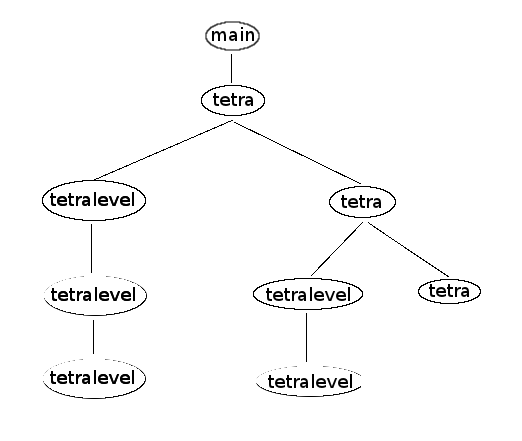
\includegraphics[width=0.45\linewidth]{graph.png}
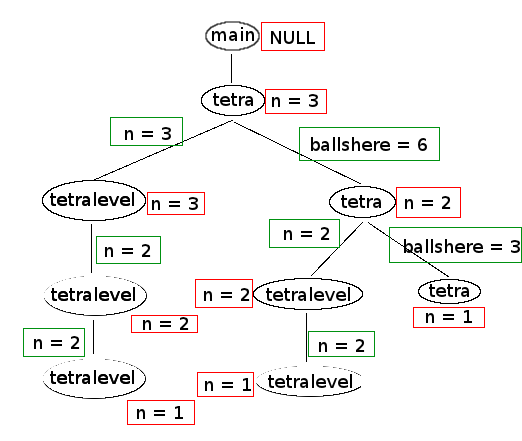
\includegraphics[width=0.45\linewidth]{state.png}


During interpretation, we build a call tree which is the data
structure we use to answer queries about the history of the program.
The call tree with no state saving information is shown above in
figure 2.  We save two types of state snapshots, each of which is a
set of bindings.  These snapshots are shown in figure 3 and the types
are differentiated by color.  The first is the local bindings that
exist in a function right after it is called, which is simply the
params zipped with the arguments.  The red boxes above correspond to
these snapshots, and they are stored once per node.  The second is the
local bindings that exist in the caller right before the callee is
called.  The green boxes correspond to these snapshots, and they are
stored once per edge.

Now, we have enough information to quickly print either the local
bindings or the entire call trace at any point in the execution of the
program.  After the programmer chooses a LOC and a specific execution
of that LOC, we map this choice to a node in the above tree.  The
local state can be quickly computed by re-executing the function up to
the query point using the stored bindings (red).  Our programs are
completely deterministic with no IO, thus we will always recompute the
same state without affecting the outside world.  Determining the full
state of the stack, including the states in the caller functions, is
as simply as walking up the tree and printing out the stored bindings
(green) at each edge.

\section{Debugging}
There are a number of commands a user can use in our debugger. Like GDB,
we support cursory inspection of source coude using
\ttt{l <line number>}. You can see the result of running the program using
\ttt{r} or \ttt{run}. To do the actual inspection you use the \ttt{s} or
\ttt{fs} commands. Both \ttt{s} and \ttt{fs} take a line number as an
argument and output either the state of the enclosing stack frame before
executing that line of source code or the entire stack at the same
point. In many programs, a single line of code is executed many times. If
it is the case that a single line of code was executed more than once, we
prompt the user to disambiguate which version of the stack they wish to
inspect (i.e. the stack corresponding to the $n$th execution of that
line).

\section{Performance}
The implementation choices we made directly trade space for time. What
this means in particular is that in MGDS, since there is no IO or
non-determinism, that to get the state of the program at any point, the
debugger could just re-run the program to that exact point. However, for a
long running program, this could take a while. With our method, we instead
save state and only replay the evaluation within a single function.

\section{Future Work}
There were numerous features that were cut in the interest of time. Arrays
were our next target and would have allowed us to implement sorting
algorithms. Support for other types besides ints was also planned.

In terms of UI, we were planning on implementing a feature that shows the
call graph of the program. Lines of code that were executed more than once
would be shown in the call graph annotated with a number. That number
would be used to uniquely identify an execution of a line of code.

We also would have like to experiment with \ttt{for} and \ttt{while}
loops, but because our UI was not great for disambiguation to begin with,
we decided it was not worth pursuing until solving the UI problems. With
\ttt{for} loops, we would need to specify the value of the loop
index. \ttt{while} loops would be harder since there are no predefined loop
variables. 

Finally, we avoided many issues by essentially architecting our language,
MGDS, to have no side effects. While we do have multiple assignment to one
variable, we don't deal with more complex issues such as IO, writing to
files, and other externally visible side-effects. Since part of our
assumption was that we could rerun a function up to a line of code in the
body, we depended on the code executing deterministically each time. If we
allow user input, random number generators, or similar, the semantics of
our debugger could be violated.

\section{Conclusions}
TODO MG

Finally, if you are interested in seeing the details of our
implementation, our code is available to be viewed on Github at
\ttt{https://github.com/dcsommer/CS240H-Final-Project} .

\section{References}
\begin{enumerate}[{[}1{]}]

\item
\ttt{http://blogs.msdn.com/b/ianhu/archive}

\ttt{/2009/05/13/historical-debugging-in-visual-studio-team-system-2010.aspx}

\item
\ttt{http://en.wikipedia.org/wiki/LR\_parsing}

\item

\end{enumerate}
\end{document}
